\documentclass[12pt,letterpaper]{article}
\usepackage{natbib}
\usepackage{layout}
\usepackage[british]{babel}
\usepackage[latin1]{inputenc}
\usepackage{amssymb}
\usepackage{amsmath}
\usepackage{textcomp}
%\usepackage{type1cm}
%\usepackage{epsf}
\usepackage{graphicx}
%\usepackage{asp2006}
%stop double-spaced lists:
%\usepackage{mdwlist}
%\doublespace
\usepackage{hyperref}
\hypersetup{colorlinks=true}
\pagestyle{plain}

%If you look into the documentation, the attributes to \titlespacing are
%command, left margin, above-skip and below-skip respectively. The *
%notation replaces the formal notation using plus/minus and etc. If you
%set it to zero, headings will snug up to the paragraphs above and below
%them:
%\usepackage[compact]{titlesec}
%\titlespacing{\section}{0pt}{*2}{*1}
%\titlespacing{\subsection}{0pt}{*2}{*1}
%\titlespacing{\subsubsection}{0pt}{*1}{*1}

%%%%%%%%%%%%%%%%%%%%%%%%%%%%%%
	\oddsidemargin  0.0in
	\evensidemargin 0.0in
	\textwidth      6.5in
	\headheight     0.0in
	\topmargin      0.0in
	\textheight=9.0in
%%%%%%%%%%%%%%%%%%%%%%%%%%%%%%

\setlength{\parskip}{-1pt}
\setlength{\parsep}{0pt}
\setlength{\headsep}{0pt}
\setlength{\topskip}{0pt}
\setlength{\topmargin}{0pt}
\setlength{\topsep}{0pt}
\setlength{\partopsep}{0pt}

%\usepackage{fancyhdr}
%\pagestyle{fancy}
%\fancyhf{}
%\fancyfoot[C]{Project \thepage\ of 5}
%\renewcommand{\headrulewidth}{0pt}
%\renewcommand{\footrulewidth}{0pt}
%%\raggedbottom
%\raggedright
%\setlength{\tabcolsep}{0in}


\newcommand{\IUE}{{\it IUE}}
\newcommand{\HST}{{\it HST}}
\newcommand{\kms}{\ifmmode {\rm km\ s}^{-1} \else km s$^{-1}$\fi}
\newcommand{\Msun}{\ifmmode {\rm M}_{\odot} \else M$_{\odot}$\fi}
\newcommand{\Lsun}{\ifmmode {\rm L}_{\odot} \else L$_{\odot}$\fi}
\newcommand{\qo}{\ifmmode q_{\rm o} \else $q_{\rm o}$\fi}
\newcommand{\Ho}{\ifmmode H_{\rm o} \else $H_{\rm o}$\fi}
\newcommand{\ho}{\ifmmode h_{\rm o} \else $h_{\rm o}$\fi}
\newcommand{\ltsim}{\raisebox{-.5ex}{$\;\stackrel{<}{\sim}\;$}}
\newcommand{\gtsim}{\raisebox{-.5ex}{$\;\stackrel{>}{\sim}\;$}}
\newcommand{\vFWHM}{\ifmmode v_{\mbox{\tiny FWHM}} \else
                    $v_{\mbox{\tiny FWHM}}$\fi}
\newcommand{\CCF}{\ifmmode F_{\it CCF} \else $F_{\it CCF}$\fi}
\newcommand{\ACF}{\ifmmode F_{\it ACF} \else $F_{\it ACF}$\fi}
\newcommand{\Halpha}{\ifmmode {\rm H}\alpha \else H$\alpha$\fi}
\newcommand{\Hbeta}{\ifmmode {\rm H}\beta \else H$\beta$\fi}
\newcommand{\Hgamma}{\ifmmode {\rm H}\gamma \else H$\gamma$\fi}
\newcommand{\Hdelta}{\ifmmode {\rm H}\delta \else H$\delta$\fi}
\newcommand{\Lya}{\ifmmode {\rm Ly}\alpha \else Ly$\alpha$\fi}
\newcommand{\Lyb}{\ifmmode {\rm Ly}\beta \else Ly$\beta$\fi}
\newcommand{\HeI}{\ifmmode {\rm He}\,{\sc i}\,\lambda5876 \else 
	          He\,{\sc i}\,$\lambda5876$\fi}
\newcommand{\HeII}{\ifmmode {\rm He}\,{\sc ii}\,\lambda4686 \else 
	           He\,{\sc ii}\,$\lambda4686$\fi}
\newcommand{\hi}{H\,{\sc i}}
\newcommand{\hii}{H\,{\sc ii}}
\newcommand{\hei}{He\,{\sc i}}
\newcommand{\heii}{He\,{\sc ii}}
\newcommand{\fe}{Fe}
\newcommand{\feii}{Fe\,{\sc ii}}
\newcommand{\feiii}{Fe\,{\sc iii}}
\newcommand{\fevi}{Fe\,{\sc vi}}
\newcommand{\fevii}{Fe\,{\sc vii}}
\newcommand{\fex}{Fe\,{\sc x}}
\newcommand{\fexi}{Fe\,{\sc xi}}
\newcommand{\fexiv}{Fe\,{\sc xiv}}
\newcommand{\neiii}{Ne\,{\sc iii}}
\newcommand{\neiv}{Ne\,{\sc iv}}
\newcommand{\nev}{Ne\,{\sc v}}
\newcommand{\ci}{C\,{\sc i}}
\newcommand{\cii}{C\,{\sc ii}}
\newcommand{\ciii}{\ifmmode {\rm C}\,{\sc iii} \else C\,{\sc iii}\fi}
\newcommand{\civ}{C\,{\sc iv}}
\newcommand{\CIV}{\ifmmode {\rm C}\,{\sc iv}\,\lambda1549 \else 
	           C\,{\sc iv}\,$\lambda1549$\fi}
\newcommand{\alii}{Al\,{\sc ii}}
\newcommand{\Ni}{N\,{\sc i}}
\newcommand{\nii}{N\,{\sc ii}}
\newcommand{\niii}{N\,{\sc iii}}
%\newcommand{\niii]}{N\,{\sc iii}]\fi}
\newcommand{\niv}{N\,{\sc iv}}
\newcommand{\nv}{N\,{\sc v}}
\newcommand{\oi}{O\,{\sc i}}
\newcommand{\oii}{O\,{\sc ii}}
\newcommand{\oiii}{O\,{\sc iii}}
\newcommand{\ob}{[O\,{\sc iii}]\,$\lambda \lambda 4959,5007$}
\newcommand{\oiv}{O\,{\sc iv}}
\newcommand{\ov}{O\,{\sc v}}
\newcommand{\ovi}{O\,{\sc vi}}
\newcommand{\mgi}{Mg\,{\sc i}}
\newcommand{\mgii}{Mg\,{\sc ii}}
\newcommand{\siiii}{Si\,{\sc iii}}
\newcommand{\siiiifb}{[Si\,{\sc iii}]}
\newcommand{\Sizw}{Si\,{\sc ii}}
\newcommand{\siiv}{Si\,{\sc iv}}
\newcommand{\si}{S\,{\sc i}}
\newcommand{\sii}{S\,{\sc ii}}
\newcommand{\siii}{S\,{\sc iii}}
\newcommand{\caii}{Ca\,{\sc ii}}
\newcommand{\cav}{Ca\,{\sc v}}
\newcommand{\aliii}{Al\,{\sc iii}}
\newcommand{\sigbl}{$\sigma_{\rm blue}$}
\newcommand{\Flamunit}{erg s$^{-1}$\,cm$^{-2}$\,\AA$^{-1}$}
\newcommand{\lam}{$\lambda$}
\begin{document}

\begin{center}
{\large SPAMM -- Spectral Properties of AGN Modeled through MCMC }
\end{center}
\vspace{0.05in}

\section*{Spectral Components}

\subsection*{Nuclear Continuum}
\begin{equation}
F_{\lambda,{\rm PL}}=F_{\rm PL,0} \ \left(\frac{\lambda}{\lambda_0}\right)^{\alpha} 
\end{equation}
where $F_{\rm PL,0}$ is the power-law normalization, $\alpha$ is the power-law slope and $\lambda_0$ is the median wavelength 
of the observed wavelength range. 

\subsubsection*{Code Parameters}
\begin{itemize}
    \item {\tt param1}: power-law slope ($\alpha_{\lambda}$)
    \item {\tt param2}: power-law normalization ($F_{\rm PL,0}$)
\end{itemize}

\subsubsection*{Priors}
\begin{itemize}
    \item {\tt $\alpha_{\lambda}$}: flat prior in range [-3,3]
    \item {\tt $F_{\rm PL,0}$}: flat prior between 0 and the maximum of the spectral flux after computing running median
\end{itemize}


\subsection*{Balmer Continuum}
If we assume gas clouds with uniform temperature $\rm{T}_{\rm{e}}$, that are partially optically thick, for wavelengths bluer 
than the Balmer edge ($\lambda_{\rm{BE}}=3646$ \AA, rest frame), the Balmer spectrum can be parametrized as 
(Grandi et al., 1982): 
\begin{equation}
F_{\lambda,{\rm BC}}= F_{{\rm BE}} \ B_{\lambda}\left({\rm T}_{{\rm e}}\right) \ \left(1-{\rm e}^{-\tau_{{\rm BE}}\left(\frac{\lambda}{\lambda_{{\rm BE}}}\right)^3}\right), \ \lambda<\lambda_{\rm{BE}}
\end{equation}
where $\rm{B}_{\lambda}(\rm{T}_{\rm{e}})$ is the Planck function at the electron temperature $\rm{T}_{\rm{e}}$, $\tau_{\rm{BE}}$ is the optical 
depth at the Balmer edge, and $\rm{F}_{\rm{BE}}$ is the normalized flux density at the Balmer edge. 

\subsubsection*{Code Parameters}
\begin{itemize}
    \item {\tt param1}: electron temperature (${\rm T}_{{\rm e}}$)
    \item {\tt param2}: optical depth at the Balmer edge ($\tau_{\rm{BE}}$)
    \item {\tt param3}: normalized flux density at the Balmer edge ($\rm{F}_{\rm{BE}}$)
\end{itemize}

\subsubsection*{Priors}
\begin{itemize}
    \item {\tt ${\rm T}_{{\rm e}}$}: flat prior in the [5,000-20,000] Kelvin range.
    \item {\tt $\tau_{\rm{BE}}$}: flat prior in the [0.1-2.0] range.    
    \item {\tt $\rm{F}_{\rm{BE}}$}: flat prior between 0 and the flux measured at $\lambda_{\rm BC,max}$, where $\lambda_{\rm BC,max}$ is the wavelength 
      corresponding to the maximum of the Balmer Continuum in the observed spectral range.       
\end{itemize}

\subsection*{High order Balmer lines}

At wavelengths $\lambda>$3646 \AA \ high order Balmer lines are merging into a pseudo continuum, yielding a smooth rise to the Balmer edge. 
Therefore, together with the continuum components, we also model high-order Balmer emission lines (up to n=50). Each high order emission line is modeled with a single 
Gaussian \textit{(Discussion: is it enough? Should we go for a Lorentzian profile?)}:
\begin{equation} F_{\lambda} = \frac{f_{\rm peak}}{\sigma \sqrt{2\pi}}e^{-\frac{1}{2}\left(\frac{\lambda - \mu}{\sigma}\right)^2},
\end{equation}

\subsubsection*{Code Parameters}
$\forall$ Gaussian component:
\begin{itemize}	
      \item{\tt param1} central wavelength ($\mu$)
      \item{\tt param2} width ($\sigma$)
      \item{\tt param3} amplitude ($f_{\rm peak}$)	    
\end{itemize}

\subsubsection*{Priors} 
\begin{itemize}
    \item {\tt Global priors for emission lines}
    \item {Fixed emission line ratios}: either from Marianne's list \textit{(under which assumptions are they computed?)}, or they can be computed using prescription 
      by Storey \& Hummer (1995), case B ($n_e=10^8-10^9 \ cm^{-3}$)        
\end{itemize}

\subsection*{FeII \& FeIII}
Linear combination of N broadened and scaled iron templates:
\begin{equation}
F_{\lambda {\rm{,Fe}}} = \sum_{\rm i=1,..N} F_{\rm{Fe,0,i}} \  {\rm FeTempl}_{\rm{\lambda,i}}(\sigma_i) 
\end{equation}		
where ${\rm FeTempl}_{\rm{\lambda,i}}$ is the iron template, $F_{\rm Fe,0,i}$ is the template normalization, 
and $\sigma_i$ is the width of the broadening kernel.

\subsubsection*{Code Parameters}
\begin{itemize}
    \item {\tt param1}: iron templates (${\rm FeTempl}_{\rm{\lambda,i}}$)
    \begin{itemize}
       \item {\tt UV template}: Vestergaard \& Wilkes (2001), (1250-3090) \AA
       \item {\tt Optical template}: V\'{e}ron-Cetty et al. (2004), (3535-7530) \AA
       \item {\tt Gap between UV and Optical template}: Beverly Wills, (3090-3534.4) \AA 
       \item {\tt Optical template}: Kovacevic et al. (2010), (4000-5400) \AA \ -- 5 separate templates (4 templates for F,G,S and P groups, 1 template for 
      I ZW1 lines) 
    \end{itemize}
    \item {\tt param2}: broadening kernel (Gaussian, Lorentzian)
    \item {\tt param3}: width of the broadening kernel ($\sigma_i$)
    \item {\tt param4}: template normalization ($F_{\rm Fe,0,i}$)  
\end{itemize}

\subsubsection*{Priors}
\begin{itemize}
    \item {\tt $\sigma_i$}: log-normal prior in the [500-20,000] km/s range. The other possibility is to have a Gaussian prior centered on the line width of \Hbeta.
    \item {\tt $F_{\rm Fe,0,i}$}: flat prior between 0 and the flux measured at $\lambda_{\rm Fe,i,max}$, where $\lambda_{\rm Fe,i,max}$ is the wavelength 
      corresponding to the maximum of the i-th iron template in the observed spectral range.
\end{itemize}

\subsection*{Host Galaxy}
Linear combination of N smoothed galaxy templates:
\begin{equation}
F_{\lambda {\rm{,Host}}} = \sum_{\rm i=1,..N} F_{\rm{Host,0,i}} \  {\rm HostTempl}_{\rm{\lambda,i}}(\sigma_*) 
\end{equation}
where ${\rm HostTempl}_{\rm{\lambda,i}}$ is the host galaxy template,
$\sigma_*$ is the stellar dispersion and $F_{\rm Host,0,i}$ is the
template normalization.\\

The stellar dispersion is currently applied according to the following
method. For a given template, increasing the velocity dispersion
implies convolving it with a broadening function. For simplicity, we
assume that this function is a Gaussian of width $\sigma_{*,\rm use} =
(\sigma_*^2 - \sigma_{*,\rm int}^2)^{1/2}$. For the moment we will
assume that $\sigma_{*,\rm int} = 0$, as we do not know the intrinsic
values for the current templates. Now, since we need to apply it in
wavelength space we can note that $P(v)\ dv = P(\lambda)\ d\lambda$
and that
\begin{equation}
  P(v;\sigma_*)\ =\ \frac{1}{\sqrt{2\pi}\sigma_*}\ \exp{\frac{-1}{2}\left(\frac{v}{\sigma_*}\right)^2},
\end{equation}
\noindent which implies that our convolution function in wavelength
space will be
\begin{equation}
  P(\lambda;\sigma_{\lambda},\lambda_0)\ =\ \frac{1}{\sqrt{2\pi}\sigma_{\lambda}}\ \exp{\frac{-1}{2}\left(\frac{\lambda-\lambda_0}{\sigma_{\lambda}}\right)^2},
\end{equation}
\noindent where $\sigma_{\lambda} = \sigma_* \lambda_0/c$. So, the
broadened template can be written as
\begin{equation}
  \rm HostTempl_{\lambda_0,i}(\sigma_{\lambda})\ =\ \int \rm HostTempl_{\lambda,i}(\sigma_{\lambda}=0)\ P(\lambda;\lambda_0,\sigma_{\lambda}) d\lambda.
\end{equation}
Now, since our template is discrete, we can write this equation as
\begin{equation}
  \rm HostTempl_{\lambda_0,i}(\sigma_{\lambda}) =  \sum_{\lambda} \rm HostTempl_{\lambda,i}(\sigma_{\lambda}=0) \int_{\lambda_{\rm Min}}^{\lambda_{\rm Max}} P(\lambda;\lambda_0,\sigma_{\lambda}) d\lambda,
\end{equation}
\noindent where $\lambda_{\rm Min}$ and $\lambda_{\rm Max}$ are the minimum and maximum wavelength of the bin. This can also be written as 
\begin{equation}
   \vec{\rm HostTempl_{i}(\sigma_{\lambda})} = \mathbf{K}\ \cdot\ \vec{\rm HostTempl_{i}(\sigma_{\lambda}=0)},
\end{equation}
\noindent where the matrix $\mathbf{K}$ is independent of the template
and holds all the terms of the convolution. For the moment the
convolution kernel is assumed to be a Gaussian, and the matrix
$\mathbf{K}$ only considers terms within 5$\sigma$ of $\lambda_0$ to
speed up the calculations.

\subsubsection*{Code Parameters}
\begin{itemize}
    \item {\tt param1}: Host galaxy templates (${\rm HostTempl}_{\rm{\lambda,i}}$) \textit{The template choice might depend on the observed wavelength range, how do we 
    prefer to implement this? (switch -- prior)}
    \begin{itemize}
       \item {\tt Option 1}: Empirical Templates of Galaxies (e.g. Kinney et al. 1996, ??)
       \item {\tt Option 2}: \textit{FUTURE DEVELOPMENT} Evolutionary stellar population synthesis models e.g. \href{http://www2.iap.fr/users/charlot/bc2003/}{Bruzal \& Charlot 2003}, 
	\href{http://adsabs.harvard.edu/abs/1997A&A...326..950F} {P\'{E}GASE} (starbursts and evolved galaxies), 
	\href{http://www.stsci.edu/science/starburst99/docs/default.htm}{Starburst99} (star-forming galaxies)    
    \end{itemize}
    \item {\tt param3}: stellar dispersion ($\sigma_*$), corresponding to the width of the smoothing kernel (Gaussian?)
\end{itemize}

\subsubsection*{Priors}
  \begin{enumerate}
  	\item {\tt $F_{\rm{Host,0,i}}$}: flat prior between 0 and the maximum of the spectral flux after computing running median
	\item {\tt $\sigma_*$}: flat prior in the [30-600] km/s range.
	\item {\tt Age}: \textit{FUTURE DEVELOPMENT, only in case of evolutionary stellar population synthesis models} 
	\item {\tt Metallicity}: \textit{FUTURE DEVELOPMENT, only in case of evolutionary stellar population synthesis models} 
  \end{enumerate}


\noindent Possible useful codes for inspection: \\
\begin{tabular}{ l | c  || l }
Code & Paper & Comments\\ \hline
\htmladdnormallink{STARLIGHT}{http://www.starlight.ufsc.br} & Cid Fernandes, R. et al. 2005, MNRAS, 358, 363 & One spectrum at a time\\
\htmladdnormallink{GANDALF}{http://star-www.herts.ac.uk/~sarzi/PaperV_nutshell/PaperV_nutshell.html} & Sarzi et al. 2006, MNRAS, 366, 1151 & Deals with 2D data\\ \hline
\end{tabular}

\subsection*{Host Galaxy Reddening}
Simple parameterization of reddening law between 0.12 -- 2.2 $\mu$m (Calzetti et al. 2000):

\begin{equation}F_o(\lambda) = F_i(\lambda)10^{-0.4A^\prime(\lambda)} = F_i(\lambda)10^{-0.4E_s(B-V)k^\prime(\lambda)},   \end{equation}

\begin{equation} E_s(B-V) = (0.44\pm0.03)E_g(B-V),  \end{equation}

\[ 
k^\prime = 
	\begin{cases}
	2.659(-1.857+1.040/\lambda) + 4.05  & :~0.63 \mu m \leq \lambda \leq 2.2\mu m \\
	2.659(-2.156+1.509/\lambda - 0.198/\lambda^2 + 0.011/\lambda^3) + 4.05 & :~0.12 \mu m \leq \lambda \leq 0.63\mu m,
	\end{cases}
\]
$F_o(\lambda)$ and $F_i(\lambda)$ are the dust-obscured and intrinsic continuum flux densities, respectivly; $A^\prime(\lambda)$ is the dust obscuration, $E_s(B-V)$ and $E_g(B-V)$ are the color excess of the stellar continuum and of the nebular emission lines.
\begin{equation} \beta = 1.9E_g(B-V)+\beta_o.  \end{equation}

\begin{figure}[htbp] %  figure placement: here, top, bottom, or page
   \centering
   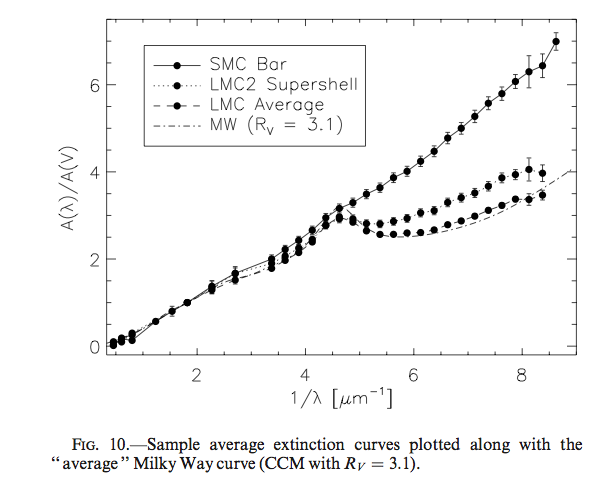
\includegraphics[width=2in]{Gordon_2003_Fig.png} 
   \caption{Gordon 2003 Plot}
   \label{fig:Gordonplot}
\end{figure}
\begin{figure}[htbp] %  figure placement: here, top, bottom, or page
   \centering
   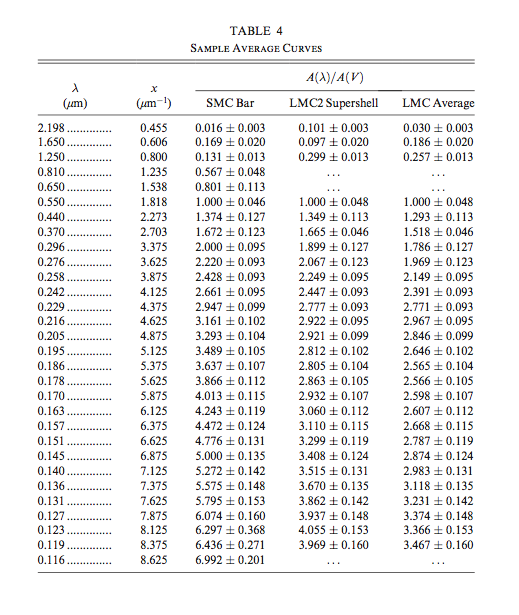
\includegraphics[width=2in]{Gordon_2003_Tab.png} 
   \caption{Gordon 2003 Table}
   \label{fig:Gordonplot}
\end{figure}
\begin{figure}[htbp] %  figure placement: here, top, bottom, or page
   \centering
   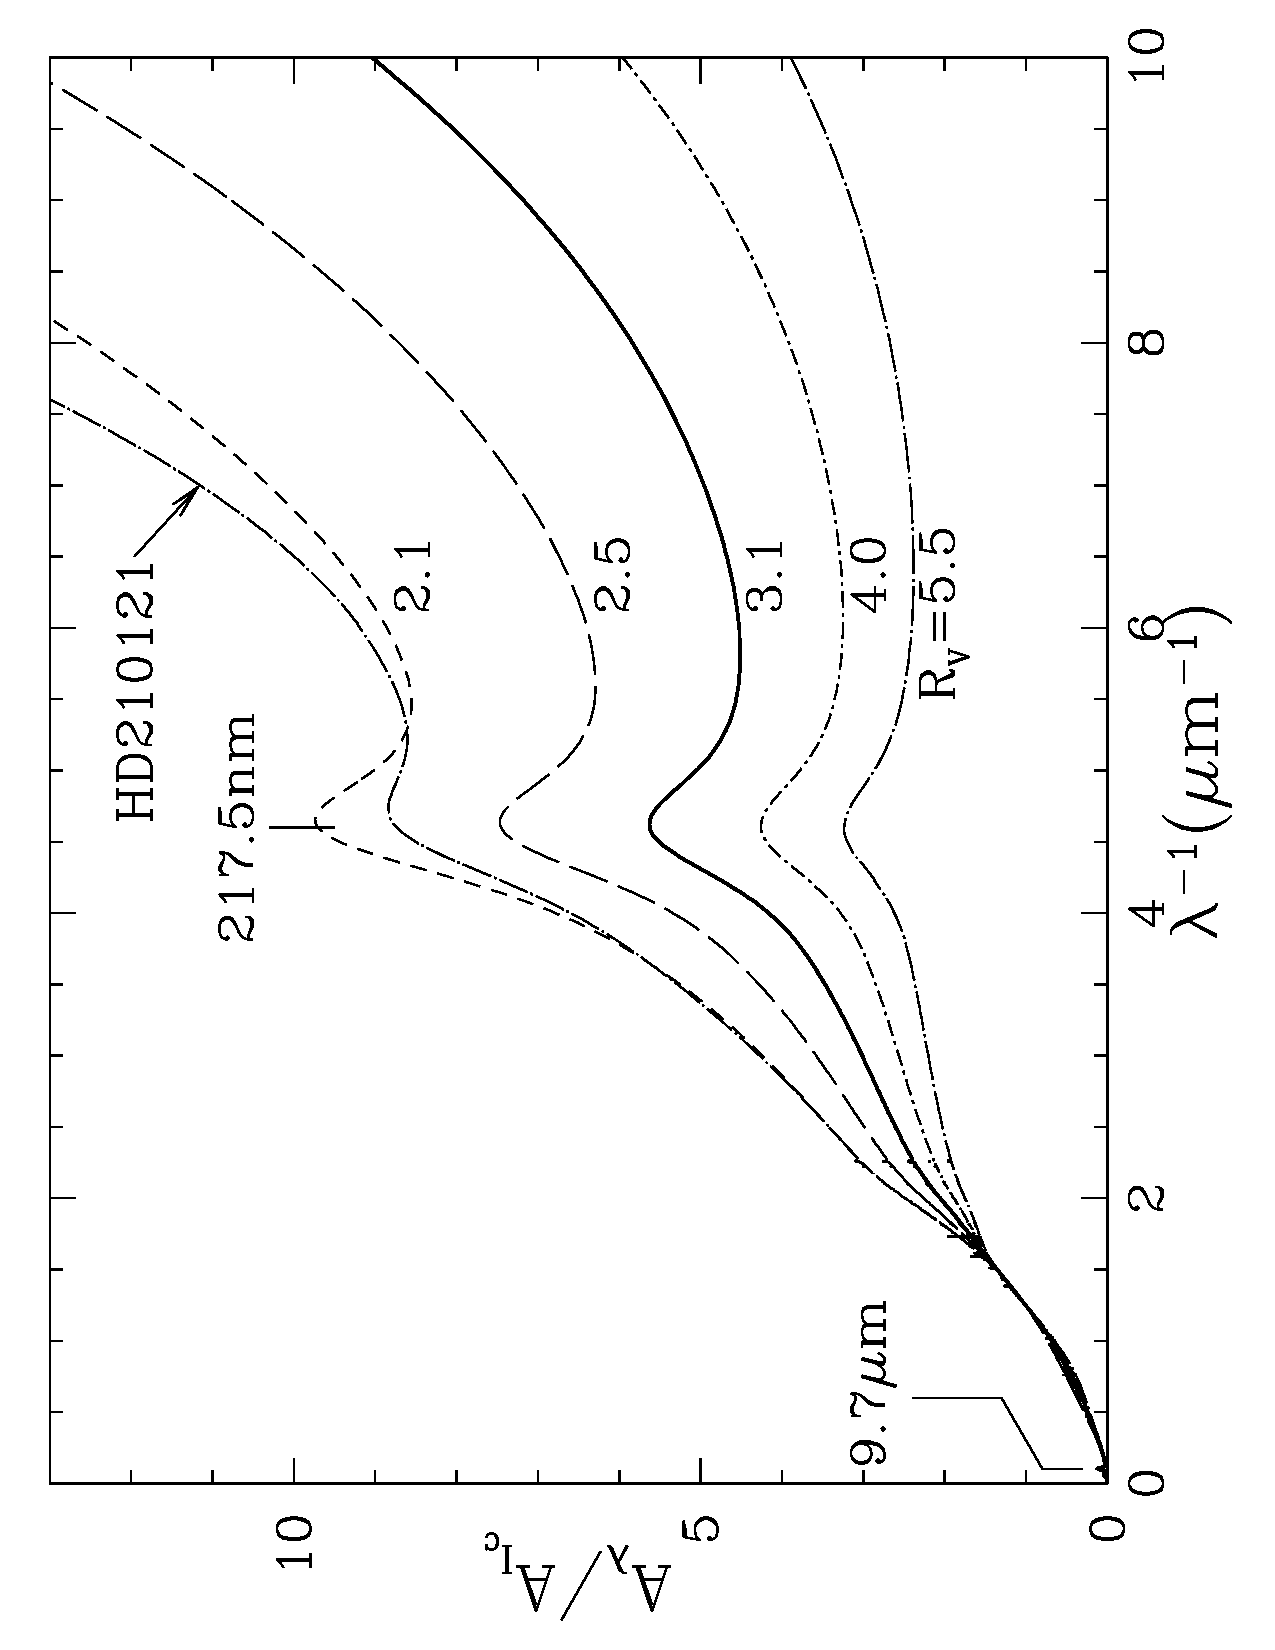
\includegraphics[width=2in]{Reddening_Draine_fig_21_2.pdf} 
   \caption{Draine 2011 Plot}
   \label{fig:Gordonplot}
\end{figure}


\subsubsection*{Code Parameters}
\begin{itemize}
    \item {\tt param1}: Possible reddening laws:
    \begin{itemize}
      \item {\tt Option 1}: Milky Way
      \item {\tt Option 2}: Large Magellanic Cloud, LMC
      \item {\tt Option 3}: Small Magellanic Cloud, SMC
      \item {\tt Option 4}: Fit for $R_v$?
    \end{itemize}
    \item {\tt param2}: Dust\_geometry: foreground screen or mixed media.
\end{itemize}

\subsubsection*{Priors}
  \begin{itemize}
   \item {\tt $\tau_{\nu}$}: flat between zero and 1.0 \textit{Discussion: do we need higher $\tau$ values?}
  \end{itemize}

\subsection*{Nuclear Reddening}

\subsubsection*{Code Parameters}
\begin{itemize}
    \item {\tt param1}: Possible reddening laws:
    \begin{itemize}
      \item {\tt Option 1}: Small Magellanic Cloud, SMC
      \item {\tt Option 2}: Fit for $R_v$?
    \end{itemize}
    \item {\tt param2}: Dust\_geometry: foreground screen or mixed media.
\end{itemize}

\subsubsection*{Priors}
  \begin{itemize}
   \item {\tt $\tau_{\nu}$}: flat between zero and 1.0 \textit{Discussion: do we need higher $\tau$ values?}
  \end{itemize}


\subsection*{Emission lines}
Functional fitting to broad and narrow emission-line components.  Each
set of ``broad'' and ``narrow'' lines will be treated as two separate
components in the code because of the relatively different sets of
priors associated with each type of line.  In addition, there are some
priors that are `global' to the type of emission lines, as a class, and
some that will be `local' to specific emission lines. Regardless of the
priors, the following functional forms will be options for fitting to
both narrow and broad emission lines.

\subsubsection*{Fitting Function Possibilities}

  \begin{itemize}
    \item Narrow Lines
      \begin{itemize}
        \item Single Gaussian with Prior (1) 
	\item Double Gaussian with Prior (1)  
        \item Option (automatically test) for additional (broader) Gaussian to \ob\ base. 
      \end{itemize}
    \item Broad Lines
      \begin{itemize}
        \item Multiple Gaussians
        \item Multiple Gauss-Hermite polynomials
        \item Gaussian (very broad) plus Gauss-Hermite (broad)
        \item Multiple Lorentzians
        \item Mix of Gaussian and Lorentzian(s) (i.e., Voigt profile)
	\item Powerlaw profiles + 1-2 Gaussians 
      \end{itemize}
   \end{itemize}

\subsubsection*{Functional Forms}
  \begin{itemize}
    \item Gaussian:
      \begin{equation} F_{\lambda} = \frac{f_{\rm peak}}{\sigma \sqrt{2\pi}}e^{-\frac{1}{2}\left(\frac{\lambda - \mu}{\sigma}\right)^2},
        \end{equation}
        where the Gaussian FWHM$=2\sqrt{2\ln 2}\sigma$ and $\mu=\lambda_0$(broad, narrow).\\

     \item $6{\rm th}$ Order Gauss-Hermite Polynomial:
       \begin{equation} F_{\lambda} = [f_{\rm peak} \alpha(w)/\sigma]\left(1 + \sum_{j=3}^{6}h_jH_j(w) \right), 
       \end{equation} 
       \begin{equation} w\equiv (\lambda - \mu)/\sigma,
       \end{equation}
       \begin{equation} \alpha(w) = \frac{1}{2\sqrt{\pi}} e^{-\frac{1}{2}w^2}. \end{equation}
       where this follows the normalization of van der Marel \& Franx (1993, ApJ, 407, 525; first equation).  The $H_j$ coefficients can be found in Cappellari et al.\ (2002, ApJ, 578, 787):
       \begin{equation} H_3(w) = \frac{w(2w^2-3)}{\sqrt{3}}, \end{equation}
       \begin{equation} H_4(w) = \frac{w^2(4w^2-12)+3}{2\sqrt{6}}, \end{equation}
       \begin{equation} H_5(w) = \frac{w[w^2(4w^2-20)+15]}{2\sqrt{15}}, \end{equation}
       \begin{equation} H_6(w) = \frac{w^2[w^2(8w^2-60)+90]-15}{12\sqrt{5}}. \end{equation}

     \item Lorentzian
       \begin{equation} F_{\lambda} = \frac{f_{\rm peak}}{\pi} \frac{\frac{1}{2}\sigma}{(\lambda - \mu)^2+(\frac{1}{2}\sigma)^2},
       \end{equation}
       where $\mu=\lambda_0$(b,n) and the Lorentzian FWHM = $\sigma = 2f_{\rm peak}/(\pi F(\mu))$.

     \item Powerlaw profile:
  \end{itemize}

\subsubsection*{Code Parameters}
\begin{itemize}
    \item $\forall$ Gaussian component:
	\begin{itemize}
	    \item{\tt param1} central wavelength ($\mu$)
	    \item{\tt param2} width ($\sigma$)
	    \item{\tt param3} amplitude ($f_{\rm peak}$)	    
	\end{itemize}

    \item $\forall$ $6{\rm th}$ Order Gauss-Hermite Polynomial:
	\begin{itemize}
	    \item{\tt param1} central wavelength ($\mu$)
	    \item{\tt param2} width of the Gaussian component($\sigma$)
	    \item{\tt param3} amplitude of the Gauss-Hermite series ($f_{\rm peak}$)
	    \item{\tt param4-7} Gauss-Hermite moments $h_3$, $h_4$, $h_5$, $h_6$
	\end{itemize}   

    \item $\forall$ Lorentzian component:
	\begin{itemize}
	    \item{\tt param1} central wavelength ($\mu$)
	    \item{\tt param2} width ($\sigma$)
	    \item{\tt param3} amplitude ($f_{\rm peak}$)	    
	\end{itemize}   

    \item $\forall$ Power-law profile:
	\begin{itemize}
	    \item{\tt param1}     
	\end{itemize}   

\end{itemize}

\subsection*{Narrow Emission lines}

\subsubsection*{Global Priors: for all i=1, N narrow lines}
\begin{itemize}

  \item $z$: flat prior between 0 and 8 with $z$=constant for all $i$ (This is the most general prior; likely, some knowledge of the redshift will be known, so in that case, this should be a Gaussian prior with much narrower width, centered on estimated redshift)
  \item $\mu/(1+z)$: flat prior between -1200 and 1200 km s$^{-1}$ with $\mu_i$ = constant for all $i$
  \item $\sigma_i$: flat prior between 0 and 1200 km s$^{-1}$ with $\sigma_i$ = constant for all $i$ {\it} (this is to fit narrow components that are co-spatial/kinematic with the ``typical'' low density NLR traced by the integrated forbidden line flux; any ``intermediate'' components will be fit with the broad emission lines.  It's also OK to go down to zero width; if the line is not found)
 \item $F_{\lambda} > 0$
 \item $F_{\rm peak}/F{\rm cont}$: flat prior with range of 0 to 10,000 (i.e, it's OK for the line not to be found)
 \item $h_j$: flat prior between -0.3 and 0.3 (KD: this is just what I used in my code for my Gauss-Hermite polynomial fits and it seemed to work OK).

\end{itemize}

\subsubsection*{\bf Narrow Emission Line List, \boldmath{$\lambda_{0,n}$}}
    \begin{itemize}
      \itemsep-0.1cm
      \item {[\nev]\, $\lambda$3425.900\AA}
      \item {[\oii]\, $\lambda \lambda$3726.000, 3728.800\AA}
        \begin{itemize}
          \item {\bf Local Prior:} doublet ratio 1:1 (actually density dependent, but the doublet is too closely spaced to constrain in AGNs; Osterbrock); flat prior in range $1:1\pm 0.3$
        \end{itemize}
      \item {[\neiii]\, $\lambda$3868.800\AA}
      \item \heii\ (actual $\lambda=4685.650$\AA) 
      \item \Hbeta\ $\lambda=4861.320$\AA
        \begin{itemize}
          \item {\bf Local Prior:} ratio of narrow \Hbeta:[\oiii]\, $\lambda$5007; flat prior in range TBD by BPT diagram results (my experience ~0-0.4:1)
        \end{itemize}
      \item {[\oiii]\, $\lambda \lambda$4958.920, 5006.850\AA}
        \begin{itemize}
        \item {\bf Local Prior:} doublet ratio 1:3 (Osterbrock); flat prior in range $1:3\pm 0.5$
        \end{itemize}
      \item {[\oiii]\, $\lambda$5007 blue component}
          \begin{itemize}
          \item {\bf Local Prior:} set very loose priors on existence,
            location and strength; if the overall region fits better
            between 4959 and 5007 with the addition of a blue component,
            go with it; I'm not sure what's relevant here for coding...
            Complicated further because must keep total [\oiii]\,
            $\lambda$5007 flux ratio with 4959.
          \end{itemize}
      \item {[\nii]\, $\lambda \lambda$6548.060, 6583.39\AA}
        \begin{itemize}
          \item {\bf Local Prior:} doublet ratio 1:3 (Osterbrock); flat prior in range $1:3\pm 0.5$
        \end{itemize}
      \item \Halpha\ $\lambda=6562.780$\AA
        \begin{itemize}
          \item {\bf Local Prior:} ratio of narrow \Halpha:[\nii]; flat prior in range TBD by BPT diagram results.
        \end{itemize}
      \item {[\Sizw]\, $\lambda \lambda$6716.420, 6730.780\AA}
        \begin{itemize}
          \item {\bf Local Prior:} doublet ratio 1.1:1 (Osterbrock); flat prior in range $1.1\pm 0.3:1$
        \end{itemize}
    \end{itemize}

**{\it Any other specific requirements related to widths or velocity offsets of individual lines should be listed as local priors.}

\subsubsection*{Additional ``Conditions'' (not really priors, so I'm not sure how they should be coded)}
\begin{itemize}
   \item As listed above; the potential presence of a blue component to
    [\oiii]\, $\lambda \lambda$4958.920, 5006.850\AA.
\end{itemize} 
\subsection*{Broad Emission lines}

\subsubsection*{Global Priors: for all i=1, N Broad lines}
\begin{itemize}

  \item $z$: solution determined from NELs applied; but broad line centers can be allowed to shift relative to this solution.
  \item $\mu/(1+z)$: flat prior between -6000 and 4000 km s$^{-1}$, independent for each broad line component.
  \item $\sigma_i$: flat prior between 0 and 12000 km s$^{-1}$; multiple
    components will account for all ``very broad'', broad, and
    ``intermediate'' components.  It's also OK to go down to zero width
    (if the line is not found).
 \item $F_{\lambda} > 0$
 \item $F_{\rm peak}/F{\rm cont}$: flat prior with range of 0 to 10,000 (i.e, it's OK for the line not to be found)
 \item $h_j$: flat prior between -0.3 and 0.3 (KD: this is just what I used in my code for my Gauss-Hermite polynomial fits and it seemed to work OK).

\end{itemize}

\subsubsection*{\bf Broad Emission Line List, \boldmath{$\lambda_{0,b}$}}
    \begin{itemize}
      \itemsep-0.1cm
      \item \Lya\, $\lambda$1215 (actual $\lambda=1215.670$\AA)
      \item \nv\, $\lambda$1240 (doublet at $\lambda \lambda$1238.808, 1242.796\AA)
      \item ``1400 Feature'': \siiv\ (doublet at $\lambda \lambda$1393.755, 1402.770\AA) plus \oiv] blend ($\lambda \lambda$1397.210, 1399.780, 1404.790, 1407.390\AA)
      \item \niv]\, $\lambda$1486 (actual $\lambda=1486.500$\AA)
      \item \CIV\ (unresolved doublet at $\lambda \lambda$1548.188, 1550.762\AA) 
      \item \heii\, $\lambda$1640 (actual $\lambda=1640.720$\AA)
      \item \heii\, $\lambda$1640 blue component
          \begin{itemize}
          \item {\bf Local Prior:} set very loose priors on existence,
            location and strength; if the overall region fits better
            between \heii\, $\lambda$1640 and \civ with the addition of
            a blue component, go with it; I'm not sure what's relevant
            here for coding... I can maybe try to come up with some
            better priors from looking at data I have, but probably best
            to just leave it loose and see how it does.
        \end{itemize}
      \item \oiii] $\lambda$1663 (doublet at $\lambda \lambda$1660.800, 1666.140\AA)
      \item \ciii]\, $\lambda$1909: actually a blend of \aliii\, $\lambda \lambda$1854.720, 1862.780\AA, \siiii]\, $\lambda=1892.030$\AA, and \ciii]\, $\lambda=1908.734$\AA.
      \item \mgii\, $\lambda$2798 (doublet at $\lambda \lambda$2796.350, 2803.530\AA)
      \item \Hdelta\ $\lambda=4101.735$\AA
      \item \Hgamma\ $\lambda=4340.450$\AA
      \item \HeII\ (actual $\lambda=4685.650$\AA) 
      \item \HeII\ blue component
          \begin{itemize}
          \item {\bf Local Prior:} set very loose priors on existence,
            location and strength; if the overall region fits better
            between \HeII\ and potential presence of \feii\ and host
            with the addition of a blue component, go with it; I'm not
            sure what's relevant here for coding... I can maybe try to
            come up with some better priors from looking at data I have,
            but probably best to just leave it loose and see how it
            does.
        \end{itemize}
      \item \Hbeta\ $\lambda=4861.320$\AA
      \item \hei\, $\lambda$4922 (actual $\lambda=4921.9$\AA)
      \item \hei\ $\lambda=5016$\AA 
      \item \hei\, $\lambda$5876 (actual $\lambda=5875.680$\AA) 
      \item \hei\, $\lambda$6678 (actual $\lambda=6678.000$\AA) 
      \item \hei\, $\lambda$7065 (actual $\lambda=7065.300$\AA) 
      \item \Halpha\ $\lambda=6562.780$\AA
    \end{itemize}

**{\it Any other specific requirements related to widths or velocity offsets of individual lines should be listed as local priors.}


\subsubsection*{Additional ``Conditions'' (not really priors, so I'm not sure how they should be coded)}
\begin{itemize}
  \item \hei\, $\lambda$4922 and \hei\ $\lambda=5016$\AA are highly
    blended with \Hbeta, [\oiii], and possibly \feii, and thereby hard to
    independently constrain.  The condition is therefore that ``if''
    \hei\, $\lambda$5876 is present in the spectrum,
    $\sigma_{4922}=\sigma_{5016}=\sigma{5876}$.
  \item As listed above; the potential presence of a blue component to
    \heii\, $\lambda$1640 and \heii\, $\lambda$4686.  We see this region
    in reverberation campaigns when no other \feii\ is present, so we
    have evidence to suggest it's there; it's just highly blended and
    somewhat low EW in single spectra.
\end{itemize} 
    
%\begin{center}
%{\Large This is my Project}
%\end{center}
%\vspace{0.1in}
%\begin{center}
%{\bf ABSTRACT}
%\end{center}




%\begin{figure}
%\plotone{figure.eps}
%\caption{}
%\end{figure}



\end{document}
